\documentclass{article}

\usepackage[final]{neurips_2019}

\usepackage[utf8]{inputenc}
\usepackage[T1]{fontenc}
\usepackage{hyperref}
\usepackage{url}
\usepackage{booktabs}
\usepackage{amsfonts}
\usepackage{amsmath}
% \usepackage{nicefrac}
% \usepackage{microtype}
\usepackage{graphicx}
\usepackage{xcolor}
% \usepackage{multirow}
\usepackage{subcaption}
\usepackage{float}

\title{
  SwishNet: NBA Shot Prediction with Spatio-Temporal GNNs
}

\author{
  Anthony Argyropoulos \\
  Department of Computer Science \\
  Stanford University \\
  \texttt{aargy@stanford.edu}
}

\begin{document}

\maketitle
\vspace{-2.5em}

% =============================================================================
\section{Introduction}
% =============================================================================

NBA shot outcomes are stochastic, but the context surrounding each shot (player positions, defensive rotations, pre-shot motion) carries predictive signal that hand-crafted tabular features can't capture. We present SwishNet, a system for predicting shot outcomes (make/miss) from SportVU player-tracking data on 87,147 shots from the 2015--16 season. The input is a spatio-temporal graph $\mathcal{G}$ built from player and ball $(x,y,z)$ positions at shot release and 2--4 preceding snapshots; the output is a predicted probability $\hat{p} \in [0,1]$ that the shot is made. We benchmark logistic regression, decision trees, and XGBoost against graph neural network approaches and conduct a systematic comparison of four GNN convolution operators, multiple readouts, and 29 hyperparameter configurations. Our best GNN, \textsc{TemporalGRU} (AUC 0.6451), separates spatial encoding (per-timestep GATv2) from temporal aggregation (GRU); a hybrid pipeline that clusters its learned embeddings via a Gaussian mixture model and augments XGBoost with the resulting soft memberships achieves AUC 0.6551, surpassing standalone XGBoost (0.6501).

% =============================================================================
\section{Related Work}
% =============================================================================

\textbf{Tabular shot prediction.}
\citet{robertson2017nba} extracted 23 hand-crafted features from the same SportVU player tracking data (nearest-defender distance, shooter velocity, game state, etc.) and fit ridge regression, decision trees, random forests, and SVMs on ${\sim}5{,}600$ shots. All models performed near chance (${\sim}56\%$ accuracy), exposing a core limitation: compressing a 10-player court into pairwise distances to the \emph{closest} defender discards help defense, screens, and spacing. Robertson explicitly called for spatio-temporal models, directly motivating our graph approach. \citet{oughali2019nba} used pre-aggregated NBA shot logs (203K shots, 2014--15) with four features (shot distance, shot clock, dribbles, defender distance), reaching 62\% accuracy with tuned XGBoost (AUC ${\approx}0.60$). Their feature-importance analysis confirmed shot distance and defender distance dominate, but shot logs cannot capture how a shot was \emph{created} (motion trajectories, screens, rotations). These approaches are interpretable and fast but face an inherent ceiling because the feature engineering must decide \emph{a priori} which interactions matter. Our baselines (LR 0.6377, XGBoost 0.6501) confirm this ceiling.

\textbf{GNNs for shot quality.}
The most directly comparable work is \citet{schmid2025context}, who built a GNN for expected shot quality on the same dataset, achieving AUC 0.6174 on ${\sim}32{,}000$ shots with sparse $k$-NN spatial edges ($k\!=\!2$) and unified spatial-temporal message passing. Their calibration analysis and t-SNE shooter embeddings are notable, but their dataset is one-third our size, sparse graphs limit the model to two neighbors, and they do not compare GNN operators or sweep hyperparameters. Our temporal GAT (AUC 0.6451) outperforms their best model, and our hybrid pipeline (0.6551) further demonstrates complementarity between learned and hand-crafted representations. \citet{gat_tcn2023} proposed GATv2-TCN for NBA player performance with a spatial-then-temporal decomposition architecturally closest to ours; their finding that performance depends on \emph{who you play against} supports our hypothesis that full defensive configuration matters.

Across published work, shot-prediction AUC clusters in 0.59--0.65, reflecting basketball's stochasticity. Our hybrid pipeline (0.6551) shows the best path forward combines learned representations with gradient-boosted trees.

% =============================================================================
\section{Dataset and Features}
% =============================================================================

\textbf{Data sources and statistics.} We use the 2015--16 NBA SportVU tracking dataset \citep{sportvu2016}: $(x,y,z)$ coordinates of 10 players and the ball at 25\,Hz across 632 games. We align tracking data with NBA play-by-play (PBP) CSV logs \citep{pbp2019kaggle} (shooter identity, make/miss labels, timestamps) and a player shooting statistics CSV from Basketball Reference \citep{bballref2016} (21 per-player metrics: FG\%, distance-bucket percentages, assist rates, etc.). Our pipeline extracts 87,147 shots (FG\% 45.8\%); GNN models use a stratified 70/20/10 split (seed 42): 61,003/17,429/8,715 examples; baselines use 5-fold stratified CV on all shots.

\begin{figure}[t]
\centering
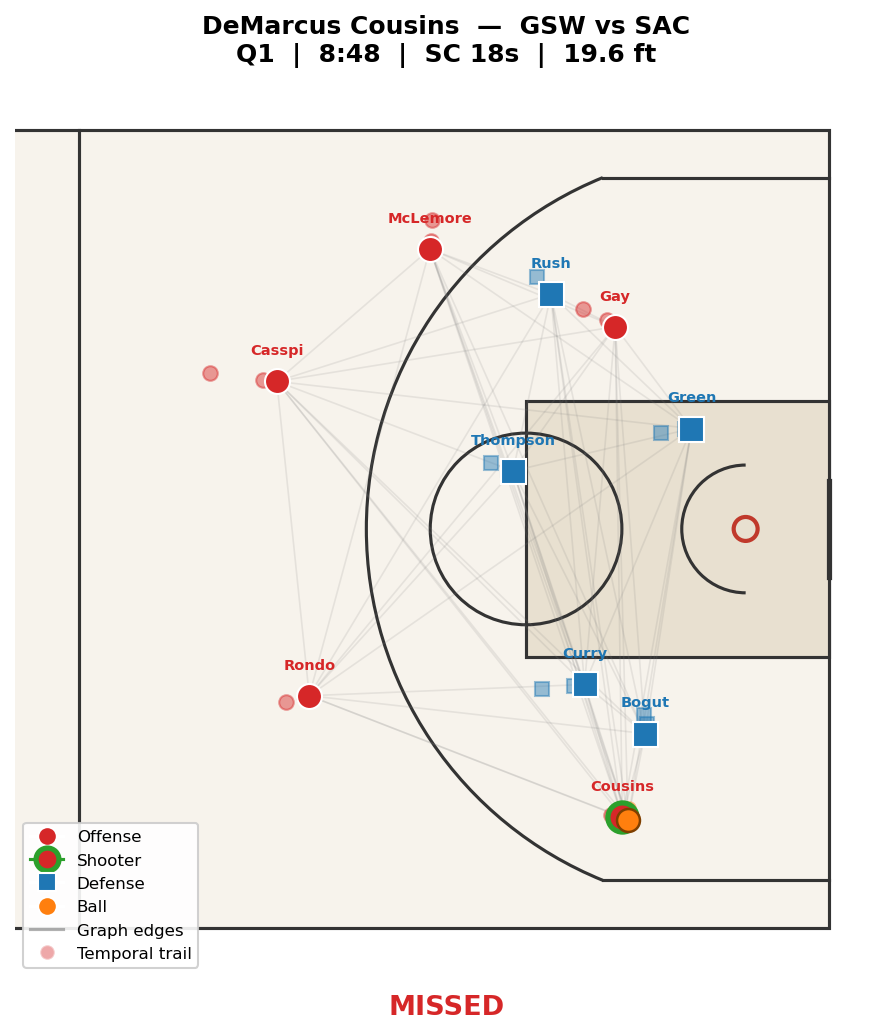
\includegraphics[height=0.26\textheight]{figures/shot_0021500468_3_cousins_missed.png}%
\hspace{0.5em}%
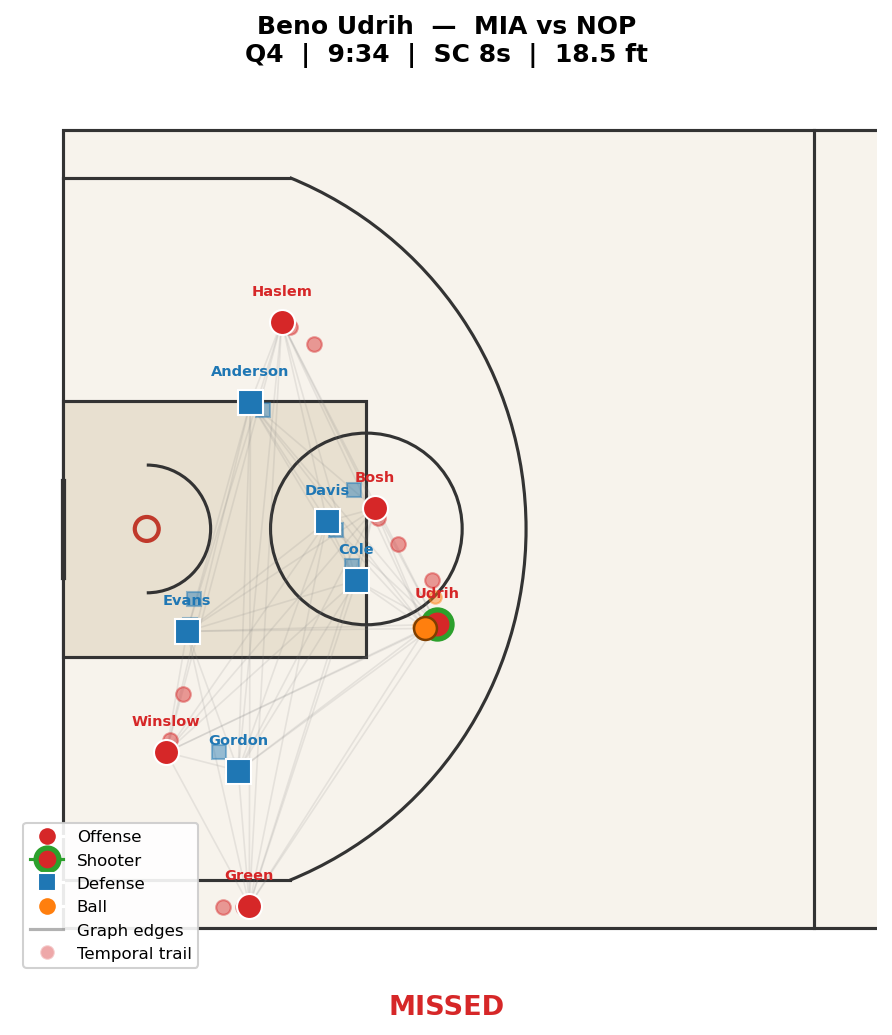
\includegraphics[height=0.26\textheight]{figures/shot_0021500436_3_udrih_missed.png}
\caption{Graph representations of two missed shots: DeMarcus Cousins' pull-up jumper, SAC vs.\ GSW (left) and Beno Udrih's mid-range jumper, MIA vs.\ NOP (right). Game footage stills: Figure~\ref{fig:game_stills}.}
\label{fig:graph_example}
\end{figure}

\textbf{Baseline feature sets.} \emph{Static-38} captures the release-frame snapshot: ball-to-rim distance, ball height, angle to basket, 3PT indicator, shot/game clocks, quarter, sorted shooter-to-teammate (4) and shooter-to-defender (5) distances, defenders within 6\,ft, and 21 shooter career statistics. \emph{Velocity-65} adds 27 motion features from the preceding frame: ball velocity and launch-angle proxy, shooter velocity, 4 teammate speeds, and per-defender velocity plus closing speed toward the shooter. No normalization is applied during feature extraction; for logistic regression we apply \texttt{StandardScaler} inside each CV fold, while tree-based models (XGBoost, decision trees) operate on raw features since they are scale-invariant.

\textbf{Shot extraction.} PBP timestamps are coarse (often offset 1--3\,s), so we locate the corresponding SportVU event within a $\pm$5\,s window and apply a physics-based algorithm: (1)~scan backward to find the \emph{rim moment} (ball within 4.0\,ft of rim center, above 9.7\,ft, descending); (2)~trace backward to the first frame where an offensive player is within 9.0\,ft of the ball, verifying identity against the PBP shooter; (3)~continue backward until ball-to-shooter distance begins increasing or drops below 6.5\,ft, identifying the release frame.

\textbf{Graph construction.} Per timestep we build 11 fully-connected nodes (5 offense, 5 defense, 1 ball; 110 directed edges) with bidirectional temporal edges across timesteps. The default samples 3 timesteps at offsets $[3, 12]$ behind release (${\sim}$0.12\,s, ${\sim}$0.48\,s), yielding 33 nodes and ${\sim}$330 edges (Figure~\ref{fig:graph_example}). Graphs with alternative timestep gaps and horizons were constructed and ablated (Table~\ref{tab:graph_variants}). Each node carries 41 \hyperlink{app:features}{features} and each edge carries 9.

% =============================================================================
\section{Methods}
% =============================================================================

\subsection{Tabular Baselines}

All tabular models are evaluated via \textbf{5-fold stratified cross-validation}: the dataset is partitioned into 5 equal folds preserving the class ratio; each fold serves once as the held-out validation set while the remaining 4 folds train the model, and the 5 validation scores are averaged. This yields a low-variance performance estimate without a fixed split.

\textbf{Logistic Regression.}
LR models $p(y\!=\!1 \mid \mathbf{x}) = \sigma(\mathbf{w}^\top\mathbf{x} + b)$ where $\sigma(z) = 1/(1+e^{-z})$. Parameters are fit by minimizing cross-entropy with optional regularization:
$\min_{\mathbf{w}} -\!\sum_i [y_i \log \hat{p}_i + (1\!-\!y_i)\log(1\!-\!\hat{p}_i)] + \lambda \|\mathbf{w}\|_p$,
where $p\!=\!1$ (Lasso/L1, promoting sparsity) or $p\!=\!2$ (Ridge/L2, shrinking coefficients). We select the regularization strength $C = 1/\lambda$ via inner 3-fold CV over $C \in \{10^{-3}, \ldots, 10^2\}$.

\textbf{XGBoost} \citep{chen2016xgboost}.
XGBoost builds an additive ensemble of $T$ shallow trees: $\hat{y}_i = \sum_{t=1}^T f_t(\mathbf{x}_i)$, trained by gradient boosting, where each tree $f_t$ fits the negative gradient (pseudo-residual) of the loss with respect to the current prediction. The objective includes an L2 regularization term on leaf weights and a tree-complexity penalty to control overfitting. We fix $T\!=\!400$, depth$\,=\!4$, learning rate $\eta\!=\!0.05$, row/column subsampling$\,=\!0.8$.

\textbf{PCA and GMM Clustering.}
We apply PCA to 256-dim GRU embeddings (extracted from our best GNN), projecting to 2 components for visualization. We then fit a Gaussian Mixture Model: $p(\mathbf{z}) = \sum_{k=1}^K \pi_k \,\mathcal{N}(\mathbf{z};\boldsymbol{\mu}_k, \boldsymbol{\Sigma}_k)$ with diagonal covariance, selecting $K\!=\!10$ via BIC (Bayesian Information Criterion, which penalizes model complexity). The resulting 10-dim soft membership vectors $[\gamma_{i1}, \ldots, \gamma_{iK}]$ are appended to Static-38 features for XGBoost, forming our hybrid pipeline.

\subsection{Graph Neural Networks}
\label{sec:gnn_arch}

A basketball court snapshot is naturally a \emph{graph}: 11 entities with pairwise spatial relationships that vary per shot. GNNs operate on such structures via \emph{message passing}: each node aggregates information from neighbors, learning relational patterns without hand-crafting which interactions matter. Shot prediction is a \textbf{graph-level} task: all architectures share $L$ message-passing layers, a graph-level readout (pooling), and a 3-layer MLP classifier. Each node $i$ starts with $\mathbf{h}_i^{(0)} \in \mathbb{R}^{41}$ (the raw node features from \S3), linearly projected to the hidden dimension. After each layer $\ell$, embeddings update to $\mathbf{h}_i^{(\ell+1)}$ (abbreviated $\mathbf{h}_i'$) by aggregating neighbor information. We sweep $L \in \{1,2,3,4\}$; best models use $L\!=\!4$.

\textbf{GATv2Conv} \citep{brody2022gatv2} computes dynamic attention coefficients over neighbors:
\begin{equation}
\textstyle \alpha_{ij} = \frac{\exp(\mathbf{a}^\top \text{LeakyReLU}(\mathbf{W}[\mathbf{h}_i \| \mathbf{h}_j \| \mathbf{e}_{ij}]))}{\sum_{k \in \mathcal{N}(i)} \exp(\mathbf{a}^\top \text{LeakyReLU}(\mathbf{W}[\mathbf{h}_i \| \mathbf{h}_k \| \mathbf{e}_{ik}]))}, \quad
\mathbf{h}_i' = \sigma\!\Big(\textstyle\sum_{j \in \mathcal{N}(i)} \alpha_{ij} \mathbf{W}\mathbf{h}_j\Big)
\label{eq:gatv2}
\end{equation}
The key difference from GATv1 is that the nonlinearity is applied \emph{after} concatenation, making attention truly dynamic: a defender's relevance depends on the receiver's state. Concretely, when updating the shooter's embedding, GATv2 learns to assign high attention $\alpha_{ij}$ to the closest defender and low attention to a weak-side player 20\,ft away, weighting their contributions accordingly. We use 4 attention heads with edge features $\mathbf{e}_{ij} \in \mathbb{R}^9$.

We also evaluate \hyperlink{app:gineconv}{GINEConv} \citep{hu2020gine}, \hyperlink{app:sageconv}{SAGEConv} \citep{hamilton2017sage}, \hyperlink{app:edgeconv}{EdgeConv} \citep{wang2019edgeconv}, different \hyperlink{app:readouts}{readouts} (methods to aggreagte node embeddings), and \hyperlink{app:losses}{loss functions} (details in Appendix).

\subsection{Temporal GRU Architecture}

Our best architecture, \textsc{TemporalGRU}, separates spatial and temporal processing. For each timestep $t$, a shared stack of $L$ GATv2 layers encodes the intra-timestep subgraph (11 nodes, 110 edges), and global mean pooling yields a snapshot embedding $\mathbf{h}_t \in \mathbb{R}^d$. The sequence (oldest to newest) is fed into a GRU \citep{cho2014gru}:
\begin{align}
\mathbf{z}_t &= \sigma(\mathbf{W}_z[\mathbf{h}_t \| \mathbf{s}_{t-1}]), \quad \mathbf{r}_t = \sigma(\mathbf{W}_r[\mathbf{h}_t \| \mathbf{s}_{t-1}]) \\
\mathbf{s}_t &= (1\!-\!\mathbf{z}_t)\odot\mathbf{s}_{t-1} + \mathbf{z}_t\odot\tanh(\mathbf{W}[\mathbf{h}_t \| \mathbf{r}_t\odot\mathbf{s}_{t-1}])
\end{align}
where $\mathbf{z}_t$, $\mathbf{r}_t$ are update and reset gates. The final hidden state $\mathbf{s}_T \in \mathbb{R}^{256}$ is classified by a 3-layer MLP. Temporal edges are removed from the graph; the GRU enforces causal ordering. All GNNs use Adam with early stopping (patience 25, max 200 epochs), BatchNorm, ReLU, and dropout after each layer.

% =============================================================================
\section{Experiments, Results, and Discussion}
% =============================================================================

\textbf{Metrics.} \textbf{AUC} (area under the ROC curve) is our primary metric: it measures how well a model \emph{ranks} shots by predicted make probability across all thresholds (0.5 = random, 1.0 = perfect). AUC is threshold-free and appropriate for our mild class imbalance (45.8/54.2\%). We also report \textbf{Accuracy} (at threshold 0.5) and \textbf{F1} for the \emph{make} class (minority). We generate ROC curves and confusion matrixes for our top models.

\subsection{Baseline Results}

% --- Table 1: All baselines ---
Table~\ref{tab:baselines} and Figure~\ref{fig:roc_baselines} (Appendix) present all tabular baselines and their ROC curves. XGBoost (AUC 0.6501) establishes the performance ceiling, outperforming the best LR by +0.012 and confirming that nonlinear feature interactions are present but inaccessible to linear models. All LR configurations cluster tightly between AUC 0.6350--0.6377, with regularization providing negligible improvement ($<$0.002); the Lasso coefficient plot (Figure~\ref{fig:lasso_coefs}) confirms that \texttt{dist\_to\_rim} and \texttt{def\_dist\_1} dominate, establishing ``where on the court'' and ``how contested'' as the two primary axes of shot difficulty. Decision trees peak at depth 7 (AUC 0.630--0.632) below LR, with textbook overfitting beyond depth 8 (Figure~\ref{fig:dt_depth}).

As a zero-shot sanity check, Gemini 2.0-Flash (AUC 0.567) and Gemini 2.5-Pro (0.529) both exceed chance but fall well below trained models ($-$0.07 to $-$0.12 vs.\ LR), validating that our baselines learn real signal beyond language priors.

\subsection{GNN Results}

We first explored readout strategies and convolution operators on a 12-game subset (1,745 shots). We tested five pooling strategies including mean$\oplus$max concatenation (which captures both the ``average'' court configuration and ``extreme'' player positions) and it dominated all others at AUC 0.5935 (Table~\ref{tab:phase1_results}, Appendix). No GNN matched the small-dataset LR baseline (0.614), pointing to \emph{data quantity} as the primary bottleneck.

\subsubsection{Full-Dataset Architecture Comparison (87,147 Shots)}

Scaling to 87,147 shots (70/20/10 split, seed 42) dramatically narrowed the GNN--LR gap, confirming the data-quantity hypothesis (Table~\ref{tab:arch_comparison}, Appendix). TemporalGRU, which separates spatial encoding (per-timestep GATv2) from temporal aggregation (GRU), achieved the best AUC of 0.6346, approaching but not yet exceeding the LR baseline (0.6377). The architecture ranking (GATv2 $>$ EdgeConv $\gg$ SAGEConv) confirmed that dynamic attention with edge features best identifies \emph{which} defenders matter; ignoring edge attributes entirely (SAGEConv, AUC 0.6094) was fatal. Focal loss hurt both top architectures under our mild class imbalance (Table~\ref{tab:loss_results}, Appendix), so we kept cross-entropy. A 29-configuration hyperparameter sweep on TemporalGRU (Table~\ref{tab:hp_sweep}, Figure~\ref{fig:hp_scatter}, Appendix) revealed that lr=$5\!\times\!10^{-4}$ and hd=256 dominated all top configs, with 3--4 GATv2 layers preferred. Full retraining of the top-3 sweep configs for 200 epochs (Table~\ref{tab:rerun_results}, Appendix) yielded our best GNN: rank03 (hd=256, nl=4, bs=512) at test AUC \textbf{0.6451}, surpassing the LR baseline by +0.0074 and confirming that \textbf{hyperparameter optimization was the single largest lever} (+0.0105 over defaults). We also ablated graph construction via a $2\!\times\!2$ factorial over temporal density and horizon (Table~\ref{tab:graph_variants}, Appendix); neither factor alone helped, but their combination (Variant~C: 5 timesteps over 2.0\,s) yielded +0.0065, though still below the HP-tuned rank03.

\subsection{Hybrid Pipeline: GNN Embeddings + GMM + XGBoost}

The GNN's best test AUC (0.6451) still trails XGBoost (0.6501) by 0.005. Rather than pursuing further GNN tuning, we asked whether the GNN's learned representations encode signal \emph{complementary} to hand-crafted features. We fit Gaussian Mixture Models ($K\!=\!10$, selected by BIC) on the full 256-dim GRU embeddings, recovering 10 recognizable NBA shot archetypes \emph{without supervision}, from at-rim dunks (cluster~2: FG\% 87.7\%, 5.7\,ft) to late-clock desperation threes (cluster~5: FG\% 28.9\%, shot clock 6.5\,s). The clusters also capture distinctions invisible to distance alone: clusters~6 and~4 are both close-range (2.7\,ft and 3.9\,ft) but differ sharply in FG\% (65.2\% vs.\ 43.7\%), reflecting uncontested putbacks vs.\ contested paint shots (Table~\ref{tab:gmm_clusters}, Figure~\ref{fig:pca_gmm}, Appendix).

Each shot's GMM soft membership vector $[\gamma_{i1}, \ldots, \gamma_{i,10}]$ provides a compact, learned summary of spatiotemporal context that hand-crafted features cannot express. Concatenating these 10 memberships with Static-38 features (yielding 48 features) and retraining XGBoost produces our best result: \textbf{AUC 0.6551} (Table~\ref{tab:hybrid_results}; confusion matrices in Figure~\ref{fig:confusion_matrices}, Appendix), surpassing XGBoost Velocity-65 (0.6501) by +0.0050 and the standalone GNN by +0.0100. The hybrid succeeds because the GNN and XGBoost extract largely \emph{orthogonal} signals: XGBoost relies on shot distance and shooter FG\%, while the GNN encodes defender rotations, shot-creation dynamics, and court configuration. The GNN's representations are strong, but its MLP classifier head is weaker than 400 boosted trees; decoupling representation learning from classification combines the best of both paradigms.

% --- Table: Summary of top results ---
\begin{table}[t]
\centering
\caption{Summary of top results across all methods (5-fold stratified CV where applicable, 87,147 shots). The hybrid pipeline (Static-38 + GMM soft memberships from GRU embeddings) achieves the best overall AUC.}
\label{tab:hybrid_results}
\small
\begin{tabular}{@{}lcccc@{}}
\toprule
\textbf{Method} & \textbf{AUC} & \textbf{Acc} & \textbf{F1} & \textbf{$\Delta$ vs.\ XGB Vel-65} \\
\midrule
\textbf{Static-38 + GMM (10 soft)} & \textbf{0.6551{\tiny$\pm$.002}} & \textbf{62.8\%} & \textbf{0.4773} & \textbf{+0.0050} \\
XGBoost Velocity-65 & 0.6501{\tiny$\pm$.003} & 62.4\% & 0.4758 & --- \\
XGBoost Static-38 & 0.6476{\tiny$\pm$.003} & 62.2\% & 0.4763 & $-$0.0025 \\
Top GNN (TemporalGRU, HP-tuned) & 0.6451 & 62.4\% & 0.4452 & $-$0.0050 \\
GAT Shooter (default HPs) & 0.6342 & 61.5\% & 0.450 & $-$0.0159 \\
LR Velocity-65 Lasso & 0.6377{\tiny$\pm$.002} & 61.2\% & 0.5198 & $-$0.0124 \\
\bottomrule
\end{tabular}
\end{table}

\subsection{Interpretability}

We investigate whether the GNN exploits relational graph structure or simply learns a nonlinear version of tabular features, using three complementary analyses: feature group ablation, input gradient saliency, and GATv2 attention weight inspection (Figure~\ref{fig:interpretability}, Appendix). We first apply PCA to the 256-dim GRU hidden states to visualize the learned embedding space. Just two principal components capture 88.4\% of variance, and the 2D projection shows makes and misses forming visibly separated distributions (Figure~\ref{fig:pca_gmm}a, Appendix), confirming the GRU encodes shot difficulty in a highly structured, low-dimensional manifold.

\textbf{Feature ablation} (Table~\ref{tab:ablation}) systematically zeros or shuffles each of the 7 feature groups and measures the resulting $\Delta$AUC drop from the full model (0.6451). Temporal ordering ($-$0.0087) and geometry ($-$0.0085) cause the largest degradation, while player career statistics ($-$0.0018) contribute the \emph{least}. This proves the GNN does more than a learned logistic regression on player quality: it derives signal from \emph{how the shot is being taken} rather than \emph{who is taking it}. This ranking is nearly the inverse of tabular baselines (dominated by \texttt{dist\_to\_rim} and shooter FG\%), explaining why the hybrid pipeline succeeds: the GNN and XGBoost extract largely orthogonal signals.

\textbf{Input gradient saliency} (Table~\ref{tab:saliency}) confirms this at the node level: shooter and ball nodes receive 3--4$\times$ larger gradients than other players, with role flags and geometry dominating over player stats within each node. \textbf{GATv2 attention weights} (Table~\ref{tab:attn_distance}) show player-ball edges receive the most attention (0.126 vs.\ 0.073 for defense-defense), with a strong proximity bias (0--6\,ft edges get $\sim$35\% more attention than 6--12\,ft). Together, these analyses confirm the GNN learns a spatiotemporal representation centered on the shooter-ball-defender triangle, prioritizing geometric relationships and motion dynamics over player identity.

% =============================================================================
\section{Conclusion and Future Work}
% =============================================================================

We presented SwishNet, a spatio-temporal GNN for NBA shot prediction. Across ${\sim}$50 configurations on 87,147 shots: (1)~data quantity is the dominant bottleneck (scaling from 1,745 to 87K shots reversed the GNN--LR gap); (2)~separating spatial (GATv2) and temporal (GRU) processing is critical; (3)~the GNN learns orthogonal signal to tabular models (temporal dynamics and geometry matter most, player stats least), enabling the hybrid pipeline (AUC 0.6551) to surpass both standalone GNN (0.6451) and XGBoost (0.6501); and (4)~HP optimization was the single largest lever (+0.0105 AUC). Future work should scale temporal context (3--5\,s windows with transformer-based attention) and explore real-time deployment for coaching analytics.

\clearpage
\section{Contributions}

Single-author project. Anthony Argyropoulos: data pipeline, graph construction, model architecture, GCP training infrastructure, all experiments/ablations, interpretability analyses, paper.

\section{Appendix: Tables and Figures}
\label{app:tables_figures}

\begin{figure}[H]
\centering
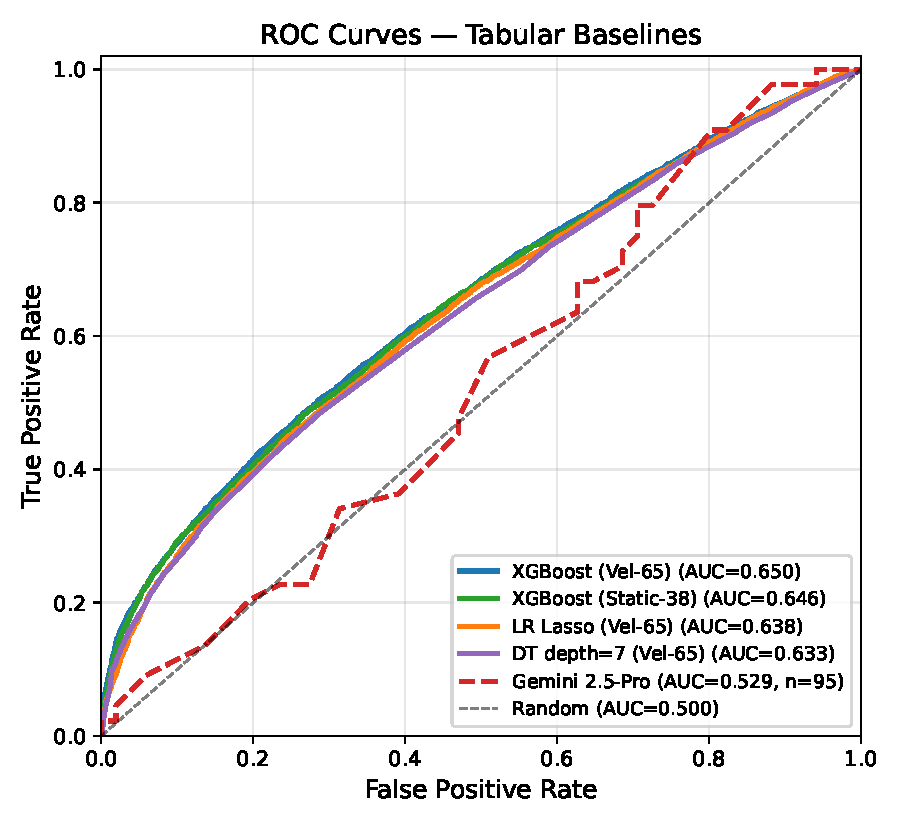
\includegraphics[width=0.85\columnwidth]{figures/baseline_roc_curves.pdf}
\caption{ROC curves for representative baselines (one CV fold). The trained models cluster tightly, all well above chance; Gemini 2.5-Pro (dashed, $n\!=\!95$) falls near the diagonal.}
\label{fig:roc_baselines}
\end{figure}

\begin{table}[H]
\centering
\caption{Tabular baseline results (5-fold stratified CV, 87,147 shots). $C^*$: regularization strength selected by inner 3-fold CV. DT: decision tree at optimal depth 7.}
\label{tab:baselines}
\small
\begin{tabular}{@{}lllccc@{}}
\toprule
\textbf{Model} & \textbf{Features} & \textbf{Config} & \textbf{AUC} & \textbf{Acc} & \textbf{F1} \\
\midrule
\multicolumn{6}{l}{\emph{XGBoost}} \\
XGBoost & Velocity-65 & depth=4, $T$=400 & \textbf{0.6501}{\tiny$\pm$.003} & 62.4\% & 0.4758 \\
XGBoost & Static-38 & depth=4, $T$=400 & 0.6480{\tiny$\pm$.003} & 62.2\% & 0.4763 \\
\midrule
\multicolumn{6}{l}{\emph{Logistic Regression}} \\
LR & Velocity-65 & Lasso, $C^*\!=\!0.1$ & 0.6377{\tiny$\pm$.002} & 61.2\% & 0.5198 \\
LR & Velocity-65 & None, scaled & 0.6376{\tiny$\pm$.002} & 61.2\% & 0.5193 \\
LR & Velocity-65 & Ridge, $C^*\!=\!1.0$ & 0.6375{\tiny$\pm$.002} & 61.2\% & 0.5193 \\
LR & Static-38 & Lasso, $C^*\!=\!0.1$ & 0.6362{\tiny$\pm$.002} & 61.0\% & 0.5194 \\
LR & Static-38 & None, raw & 0.6350{\tiny$\pm$.002} & 61.0\% & 0.5176 \\
\midrule
\multicolumn{6}{l}{\emph{Decision Tree}} \\
DT & Velocity-65 & depth=7 & 0.6318{\tiny$\pm$.002} & 61.2\% & 0.4355 \\
DT & Static-38 & depth=7 & 0.6299{\tiny$\pm$.003} & 61.3\% & 0.4354 \\
\midrule
\multicolumn{6}{l}{\emph{LLM zero-shot}} \\
Gemini 2.0-Flash & 100 shots & zero-shot & 0.5665 & --- & --- \\
Gemini 2.5-Pro & 95 shots & zero-shot & 0.5287 & 54.7\% & 0.0851 \\
\bottomrule
\end{tabular}
\end{table}

\begin{table}[H]
\centering
\caption{Phase 1 GNN results (12 games, 1,745 shots). No GNN variant matched the LR baseline (0.614).}
\label{tab:phase1_results}
\small
\begin{tabular}{@{}llcc@{}}
\toprule
\textbf{Model} & \textbf{Readout / Conv} & \textbf{Test AUC} & \textbf{Best Epoch} \\
\midrule
\multicolumn{4}{l}{\emph{Exp 1: Pooling strategies (GATv2, CE loss)}} \\
GAT mean$\oplus$max & concat(mean, max) & \textbf{0.5935} & 3 \\
GAT sum & global sum & 0.5050 & 7 \\
GAT mean & global mean & 0.4755 & 9 \\
GAT max & global max & 0.4739 & 54 \\
\midrule
\multicolumn{4}{l}{\emph{Exp 2: Shooter-centric \& GINE}} \\
GINE mean & global mean & 0.5370 & 1 \\
GAT shooter & shooter + scene mean & 0.5238 & 58 \\
GINE shooter & shooter + scene mean & 0.4854 & 3 \\
\midrule
\multicolumn{4}{l}{\emph{Baseline}} \\
LR (Static-38, Lasso) & --- & 0.6140 & --- \\
\bottomrule
\end{tabular}
\end{table}

\begin{table}[H]
\centering
\caption{Architecture comparison on full dataset (87,147 shots, default HPs). Dashed line: LR Lasso baseline (0.6377).}
\label{tab:arch_comparison}
\small
\begin{tabular}{@{}llcccc@{}}
\toprule
\textbf{Model} & \textbf{Key Design Choice} & \textbf{Test AUC} & \textbf{Acc} & \textbf{F1} & \textbf{Best Ep} \\
\midrule
TemporalGRU & spatial-then-temporal & \textbf{0.6346} & 61.2\% & 0.486 & 86 \\
GAT shooter & shooter + scene mean & 0.6342 & 61.5\% & 0.450 & 63 \\
EdgeConv & relative geometry & 0.6311 & 61.8\% & 0.483 & 65 \\
GAT mean$\oplus$max & concat(mean, max) & 0.6226 & 57.5\% & 0.172 & 71 \\
SAGEConv & mean agg, no edge feat & 0.6094 & 55.9\% & 0.143 & 35 \\
\bottomrule
\end{tabular}
\end{table}

\begin{table}[H]
\centering
\caption{Focal loss ($\gamma\!=\!1.0$) vs.\ cross-entropy on the two best architectures.}
\label{tab:loss_results}
\small
\begin{tabular}{@{}llcc@{}}
\toprule
\textbf{Model} & \textbf{Loss} & \textbf{Test AUC} & \textbf{$\Delta$ vs.\ CE} \\
\midrule
TemporalGRU & Focal $\gamma$=1.0 & 0.6304 & $-$0.0042 \\
TemporalGRU & CE (baseline) & 0.6346 & --- \\
\midrule
GAT mean$\oplus$max & Focal $\gamma$=1.0 & 0.6210 & $-$0.0016 \\
GAT mean$\oplus$max & CE (baseline) & 0.6226 & --- \\
\bottomrule
\end{tabular}
\end{table}

\begin{table}[H]
\centering
\caption{Top 10 of 29 hyperparameter configurations (sorted by validation AUC, 60-epoch sweep).}
\label{tab:hp_sweep}
\small
\begin{tabular}{@{}ccccccc@{}}
\toprule
\textbf{Rank} & \textbf{Val AUC} & \textbf{hd} & \textbf{nl} & \textbf{do} & \textbf{lr} & \textbf{bs} \\
\midrule
1  & 0.6487 & 256 & 3 & 0.1 & 5e-4 & 512 \\
2  & 0.6479 & 256 & 3 & 0.1 & 5e-4 & 256 \\
3  & 0.6477 & 256 & 4 & 0.1 & 5e-4 & 512 \\
4  & 0.6471 & 256 & 4 & 0.2 & 5e-4 & 512 \\
5  & 0.6468 & 256 & 4 & 0.1 & 5e-4 & 256 \\
6  & 0.6465 & 256 & 3 & 0.2 & 5e-4 & 512 \\
7  & 0.6462 & 128 & 3 & 0.1 & 5e-4 & 512 \\
8  & 0.6460 & 128 & 4 & 0.1 & 5e-4 & 256 \\
9  & 0.6459 & 128 & 3 & 0.1 & 5e-4 & 256 \\
10 & 0.6458 & 256 & 3 & 0.2 & 5e-4 & 256 \\
\bottomrule
\end{tabular}
\end{table}

\begin{figure}[H]
\centering
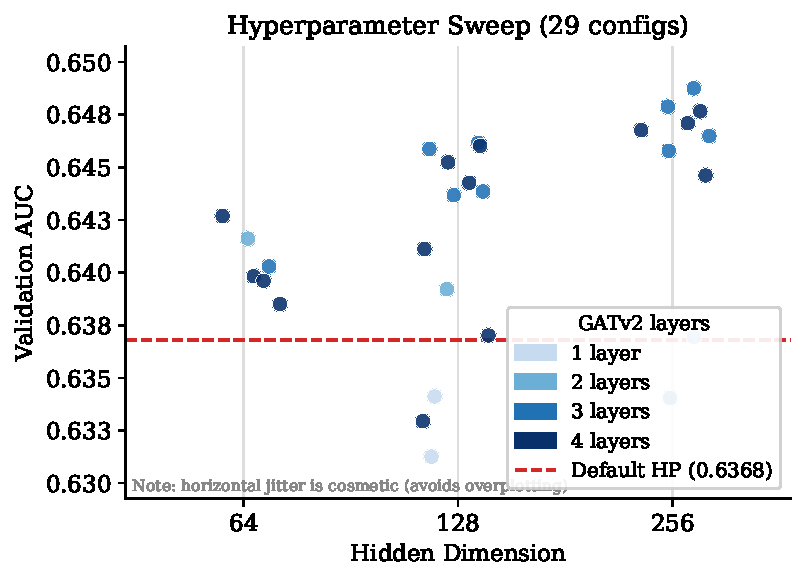
\includegraphics[width=0.85\textwidth]{figures/hp_sweep_scatter.pdf}
\caption{Validation AUC vs.\ hidden dimension for all 29 sweep configs, colored by layer count. Dashed line: default-HP baseline.}
\label{fig:hp_scatter}
\end{figure}

\begin{table}[H]
\centering
\caption{Full retraining of top-3 sweep configs (200 epochs, patience=25, L4 GPU). The third-ranked sweep config (rank03: hd=256, nl=4, bs=512) achieves the best GNN test AUC of 0.6451, surpassing the LR baseline (0.6377) by +0.0074. The sweep's top-ranked config (rank01) placed last after full training, illustrating that 60-epoch validation AUC is a noisy proxy for converged test performance. The validation--test gap averages just 0.0015, indicating minimal overfitting.}
\label{tab:rerun_results}
\small
\begin{tabular}{@{}cccccccccc@{}}
\toprule
\textbf{Config} & \textbf{hd} & \textbf{nl} & \textbf{bs} & \textbf{Sweep Val} & \textbf{Val AUC} & \textbf{Test AUC} & \textbf{Acc} & \textbf{F1} & \textbf{Best Ep} \\
\midrule
rank01 & 256 & 3 & 512 & 0.6487 & 0.6452 & 0.6437 & 62.3\% & 0.4691 & 34 \\
rank02 & 256 & 3 & 256 & 0.6479 & 0.6467 & 0.6444 & 62.3\% & 0.4200 & 59 \\
\textbf{rank03} & \textbf{256} & \textbf{4} & \textbf{512} & \textbf{0.6477} & \textbf{0.6457} & \textbf{0.6451} & \textbf{62.4\%} & \textbf{0.4452} & \textbf{49} \\
\bottomrule
\end{tabular}
\end{table}

\begin{table}[H]
\centering
\caption{Graph construction ablation ($2\!\times\!2$ factorial, rank03 HPs) varying temporal density (3 vs.\ 5 timesteps) and horizon (0.48\,s vs.\ 2.0\,s). Neither factor alone produces meaningful improvement (+0.0004 and +0.0002), but their combination (Variant~C) yields +0.0065---a striking interaction effect. The synergy arises because denser sampling within a short window adds redundancy, while a longer horizon with sparse sampling misses fine-grained motion; only together does the GRU see the full shot-creation sequence at sufficient temporal resolution. Variant~C still does not surpass rank03 (0.6451), confirming HP tuning is a larger lever than graph structure.}
\label{tab:graph_variants}
\small
\begin{tabular}{@{}llcccc@{}}
\toprule
\textbf{Variant} & \textbf{Offsets} & \textbf{Timesteps} & \textbf{Window} & \textbf{Nodes} & \textbf{Test AUC} \\
\midrule
Baseline & $[3, 12]$ & 3 & 0.48s & 33 & 0.6346 \\
A: dense\_short & $[3, 6, 9, 12]$ & 5 & 0.48s & 55 & 0.6350 \\
B: sparse\_long & $[12, 50]$ & 3 & 2.0s & 33 & 0.6348 \\
\textbf{C: dense\_long} & $[6, 12, 25, 50]$ & \textbf{5} & \textbf{2.0s} & \textbf{55} & \textbf{0.6411} \\
\bottomrule
\end{tabular}
\end{table}

\begin{figure}[H]
\centering
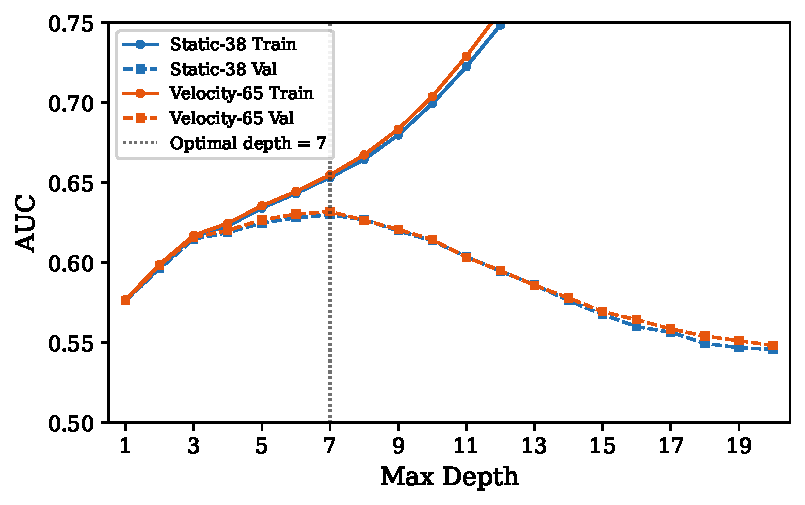
\includegraphics[width=0.85\textwidth]{figures/decision_tree_depth_curve.pdf}
\caption{Decision tree train vs.\ validation AUC by max depth (5-fold CV). Both feature sets peak at depth 7. Divergence beyond depth 8 is a textbook overfitting signature.}
\label{fig:dt_depth}
\end{figure}

\begin{figure}[H]
\centering
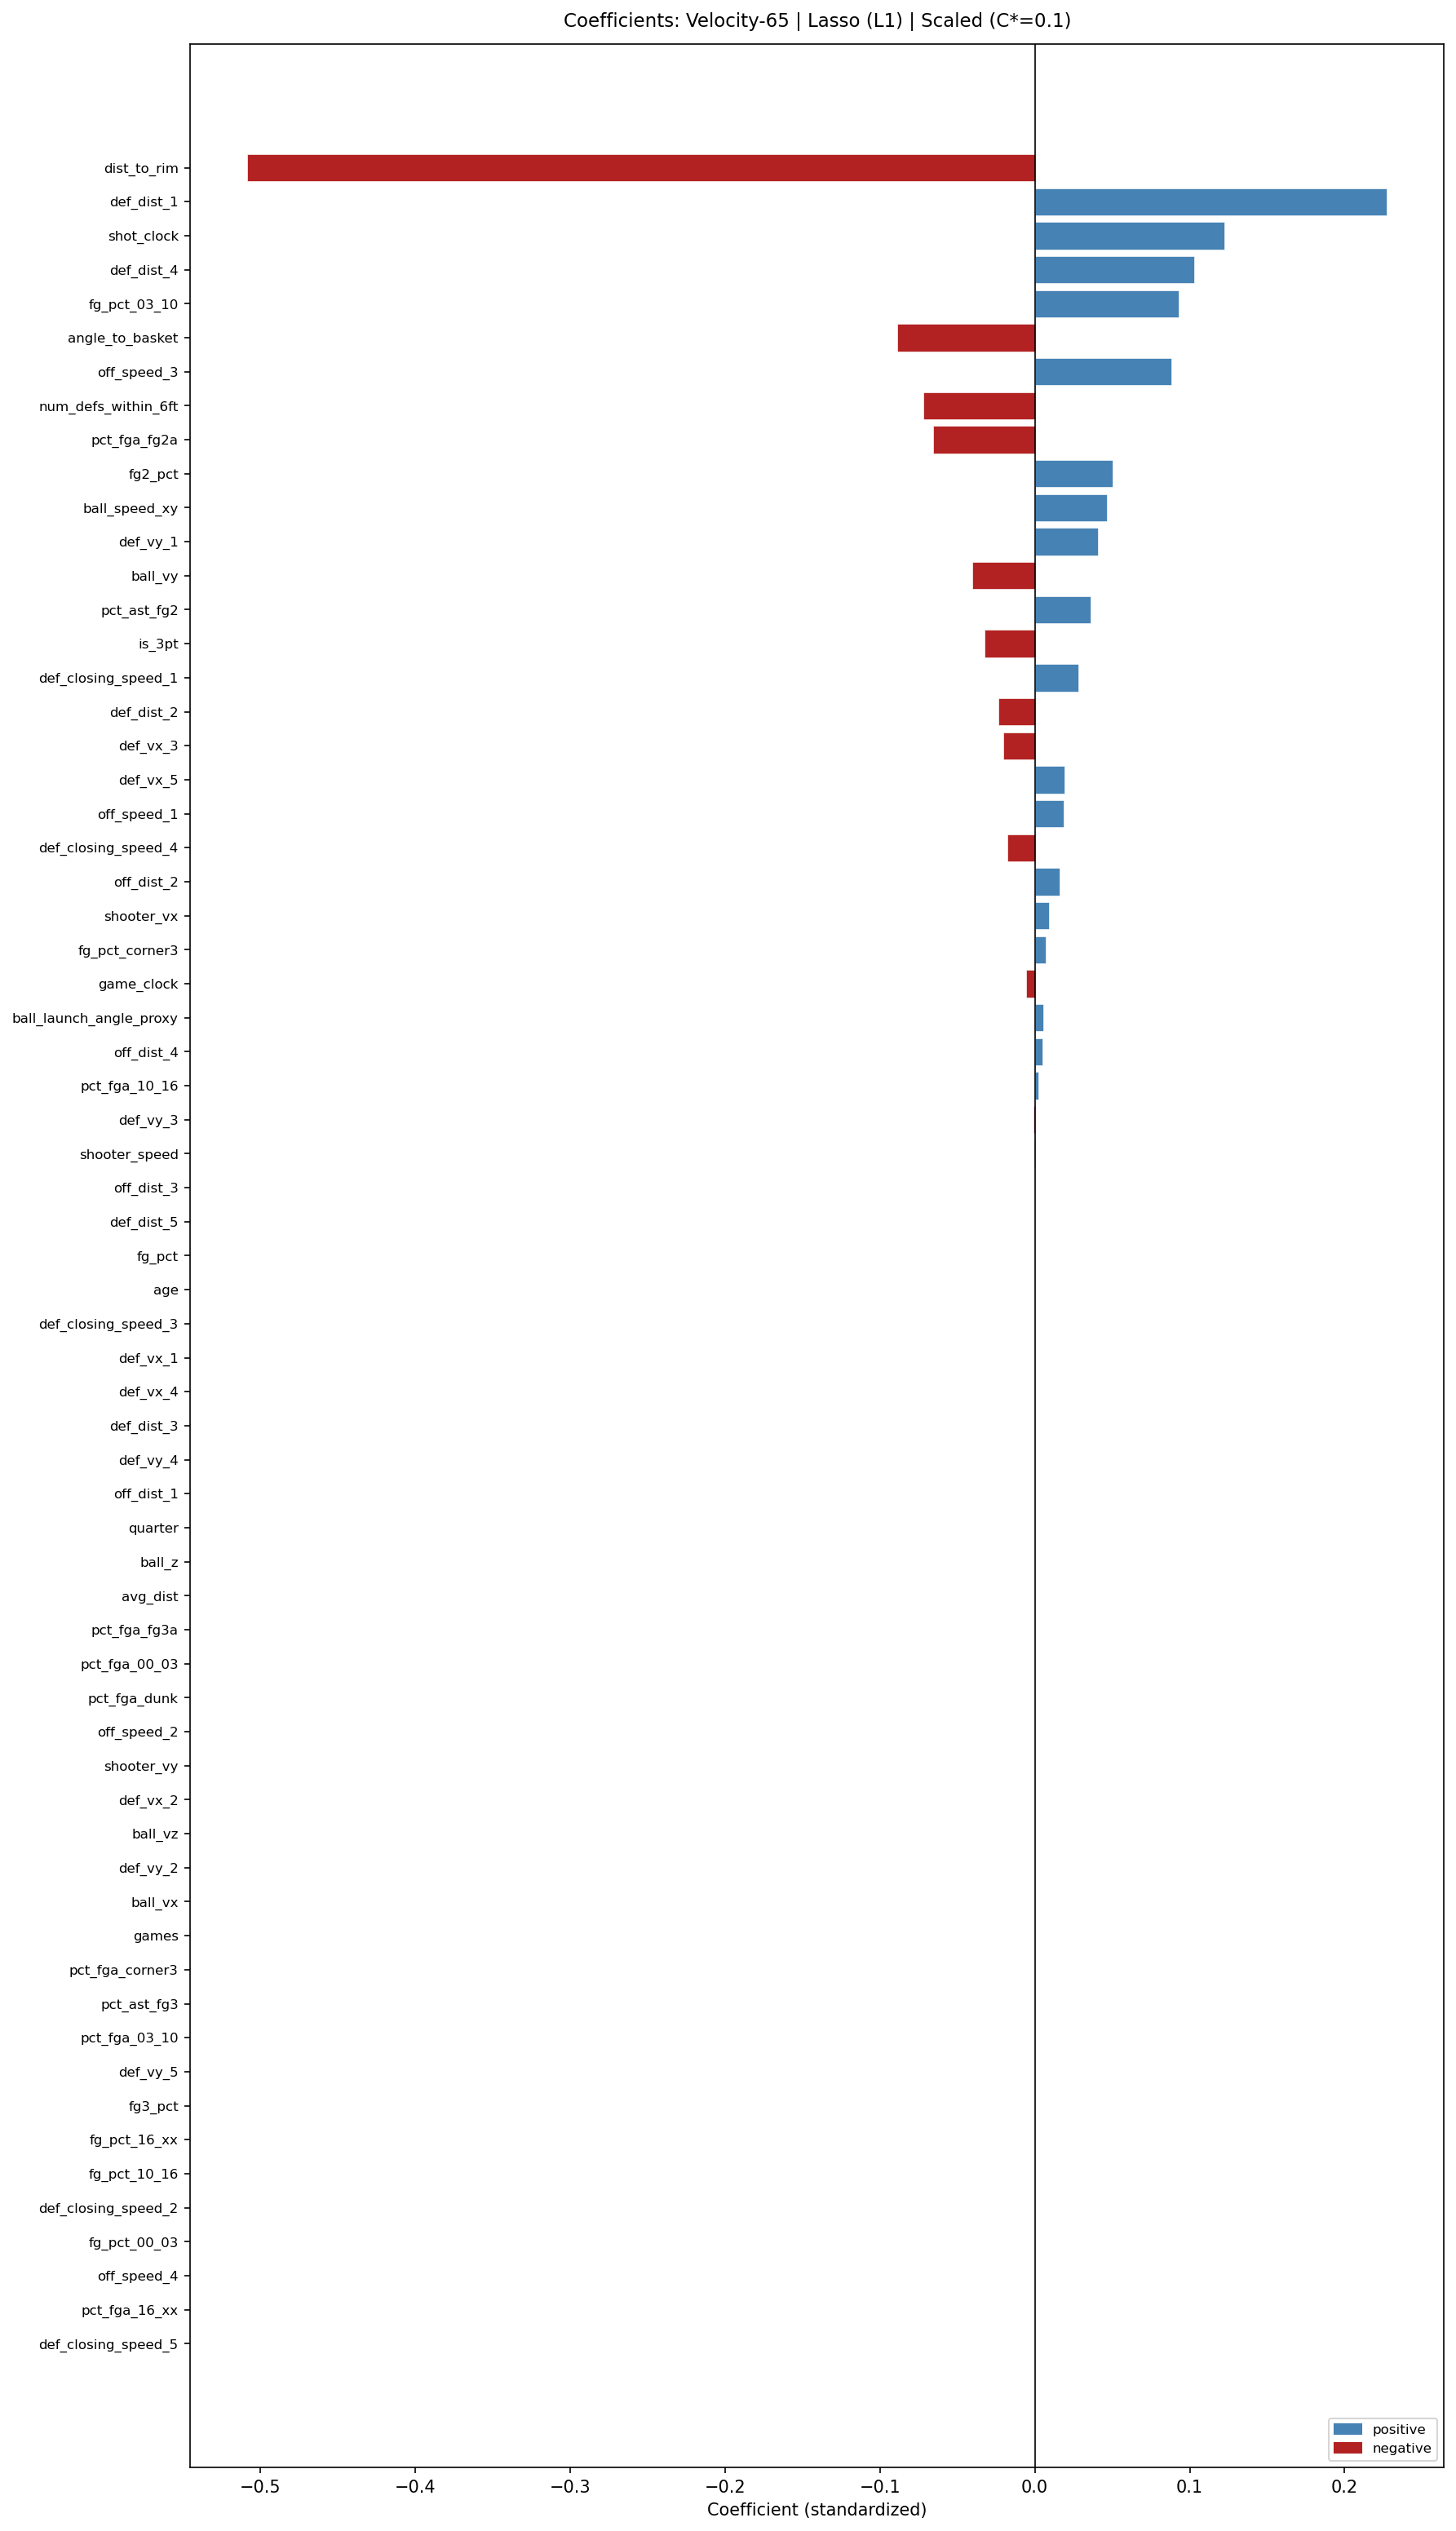
\includegraphics[width=0.75\textwidth]{figures/weights_velocity_lasso.png}
\caption{Lasso (L1) standardized coefficients on Velocity-65. \texttt{dist\_to\_rim} (negative: closer shots are easier) and \texttt{def\_dist\_1} (positive: farther defender is easier) dominate; shot-zone FG\% and \texttt{angle\_to\_basket} form the second tier; most velocity and distant-defender features are shrunk to zero.}
\label{fig:lasso_coefs}
\end{figure}

\begin{figure}[H]
\centering
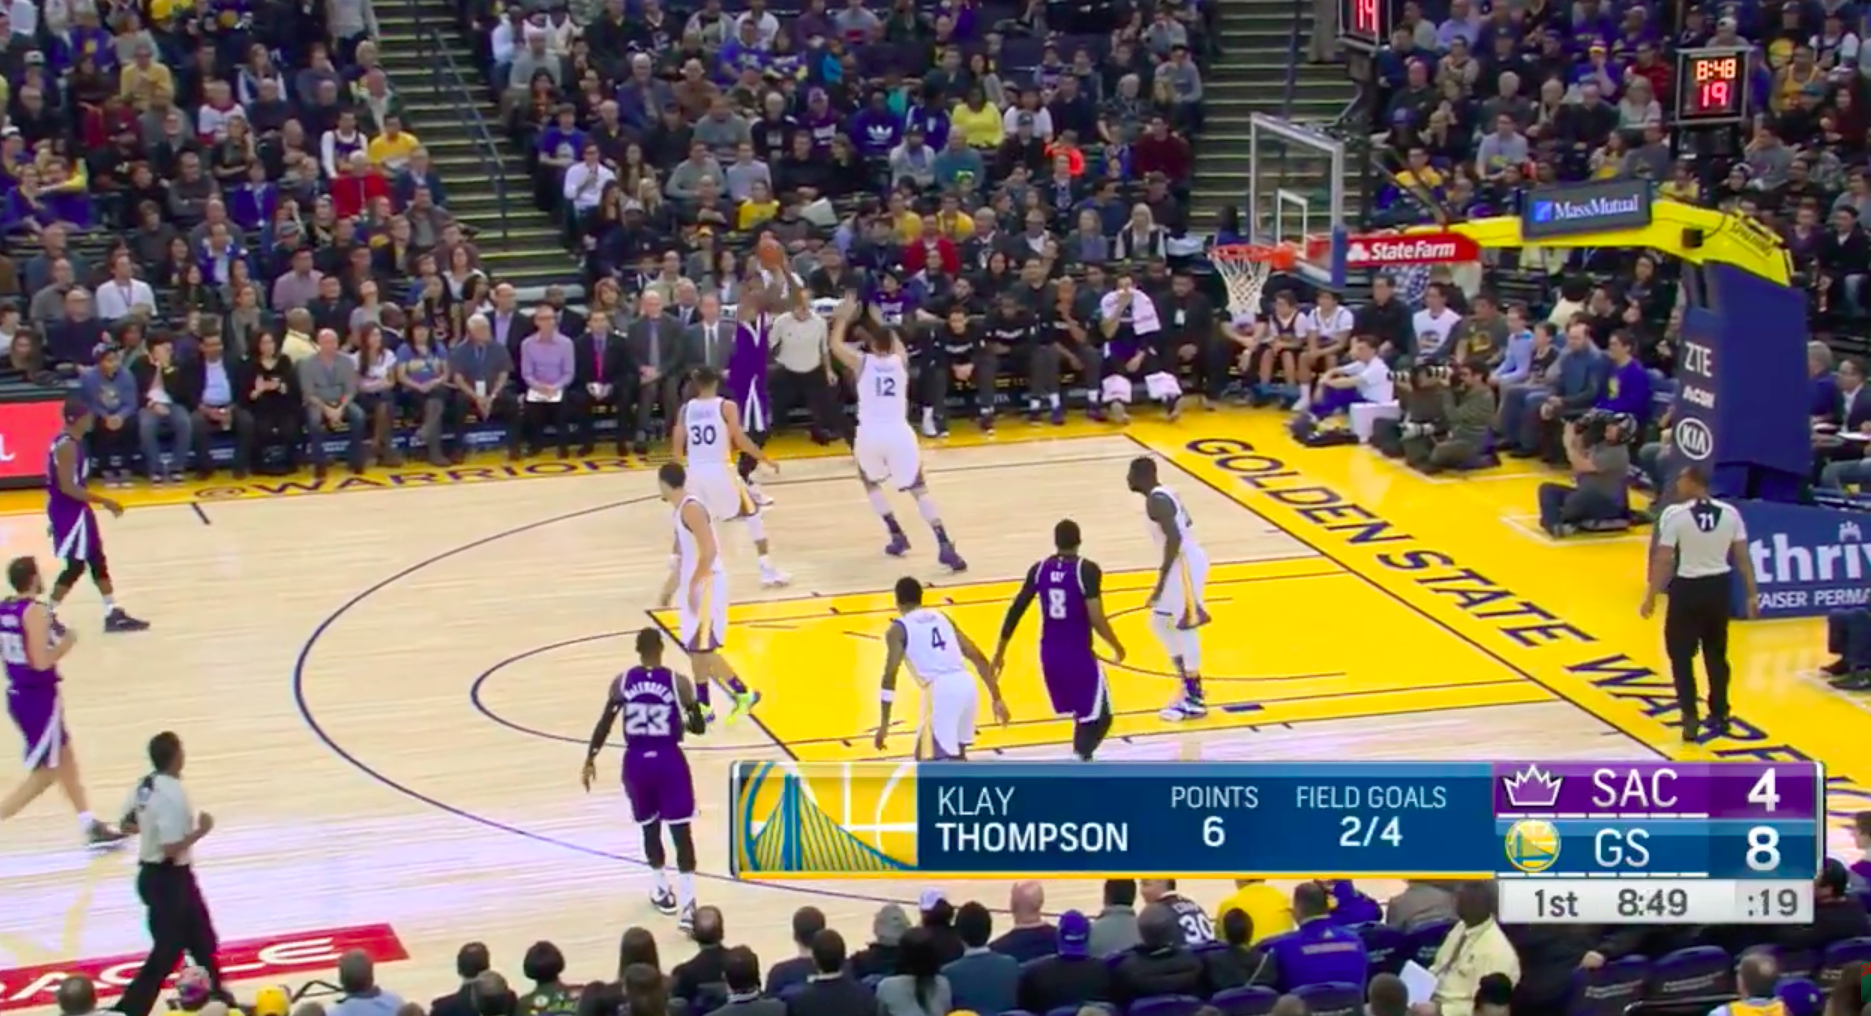
\includegraphics[width=0.46\textwidth]{figures/cousins_miss.png}%
\hfill%
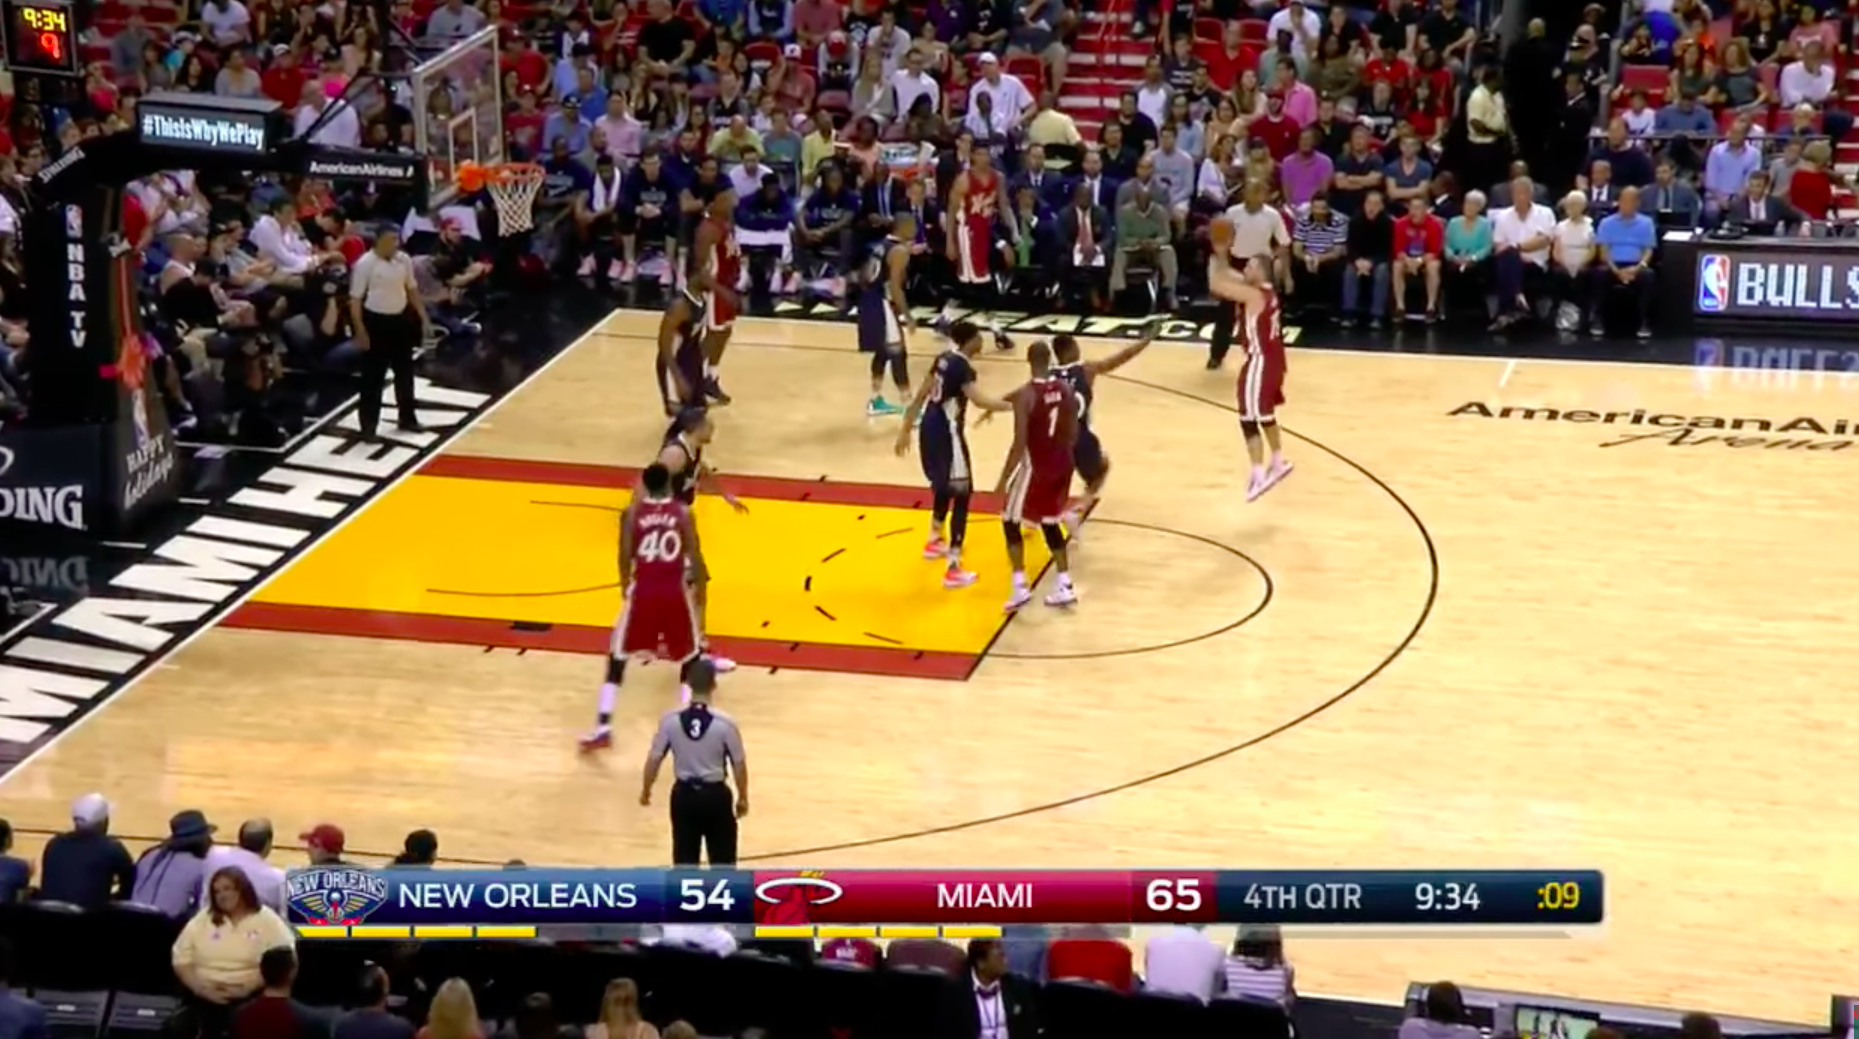
\includegraphics[width=0.46\textwidth]{figures/udrih_missed.png}
\caption{Game footage stills corresponding to the graph representations in Figure~\ref{fig:graph_example}: DeMarcus Cousins' pull-up jumper, SAC vs.\ GSW, 12/28/2015 (left) and Beno Udrih's mid-range jumper, MIA vs.\ NOP (right).}
\label{fig:game_stills}
\end{figure}

\begin{figure}[H]
\centering
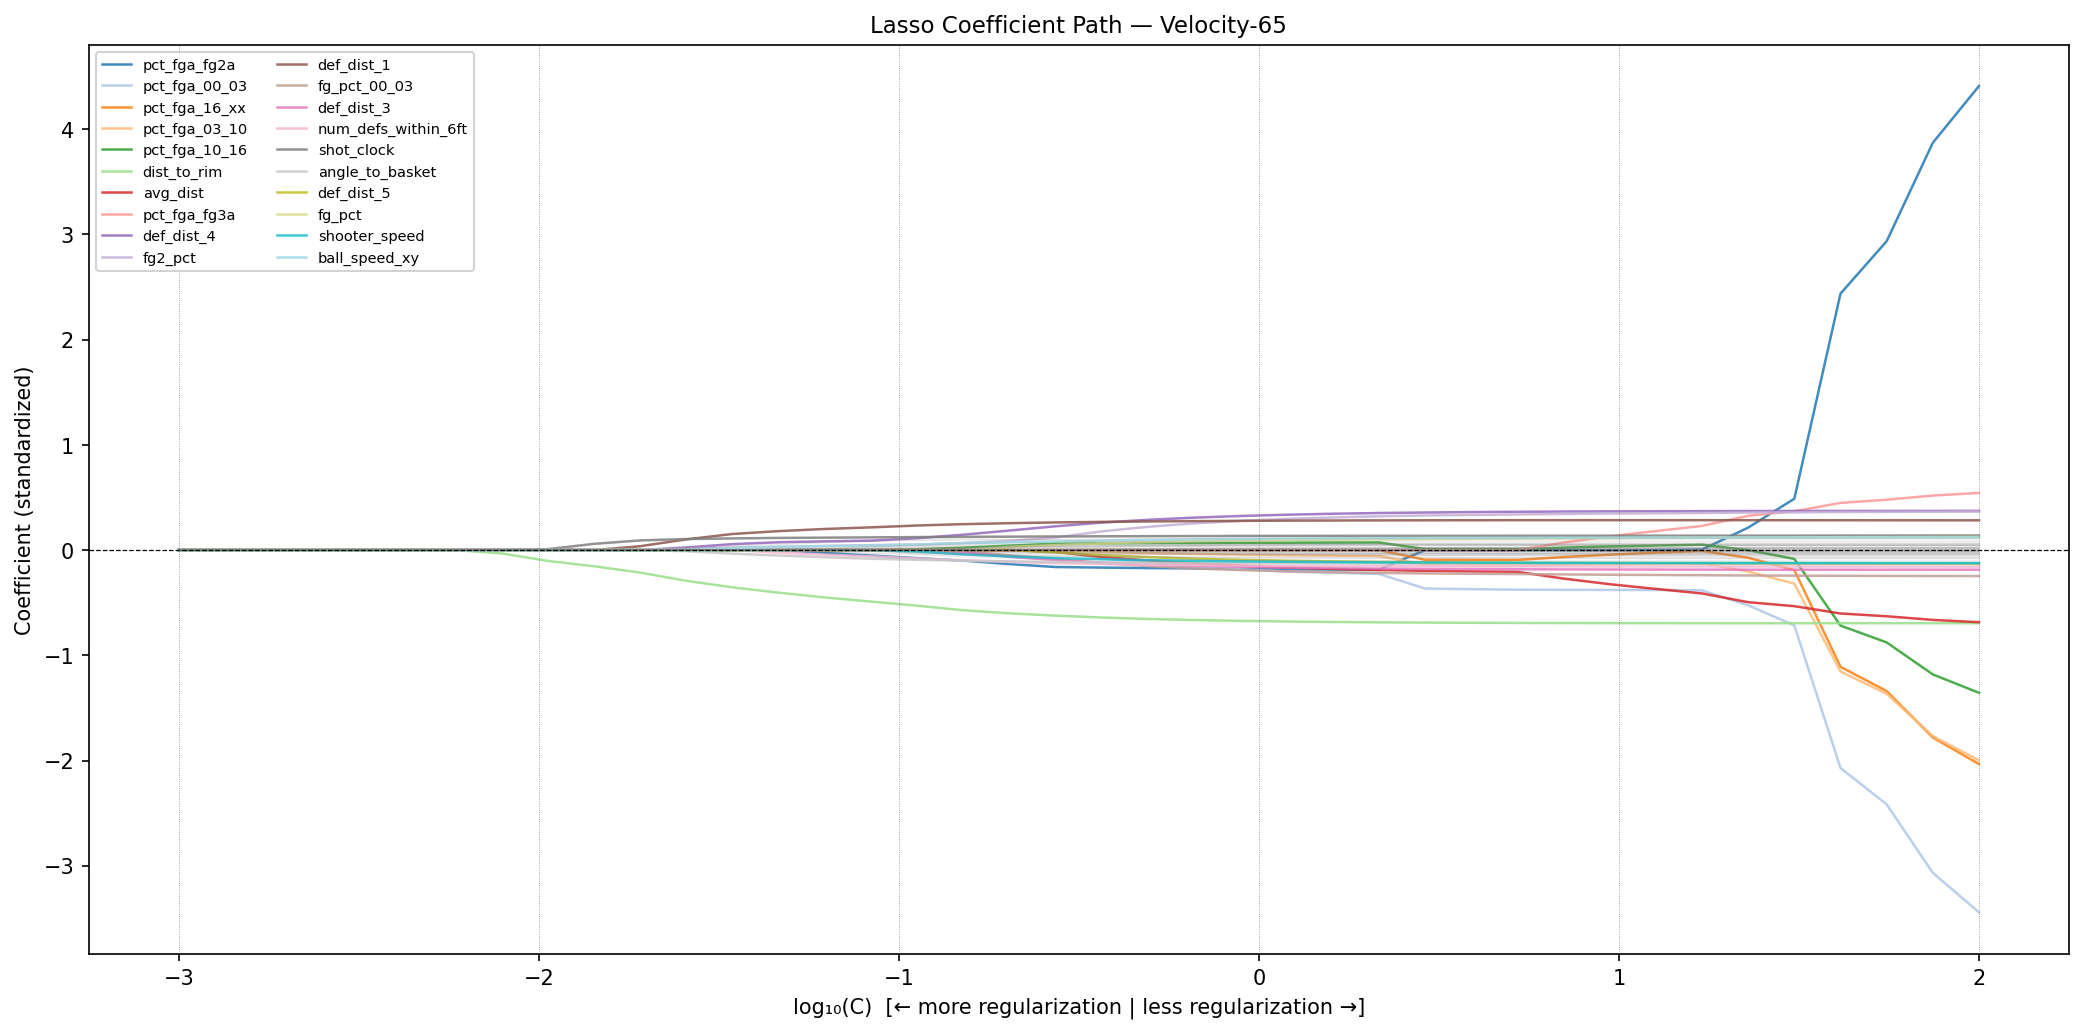
\includegraphics[width=0.85\textwidth]{figures/lasso_path_velocity.png}
\caption{Lasso regularization path (Velocity-65). As $C$ increases (less regularization), \texttt{dist\_to\_rim} and shot-zone percentages enter first, confirming they carry the strongest signal. Most velocity features remain near zero across all $C$ values.}
\label{fig:lasso_path}
\end{figure}

\begin{figure}[H]
\centering
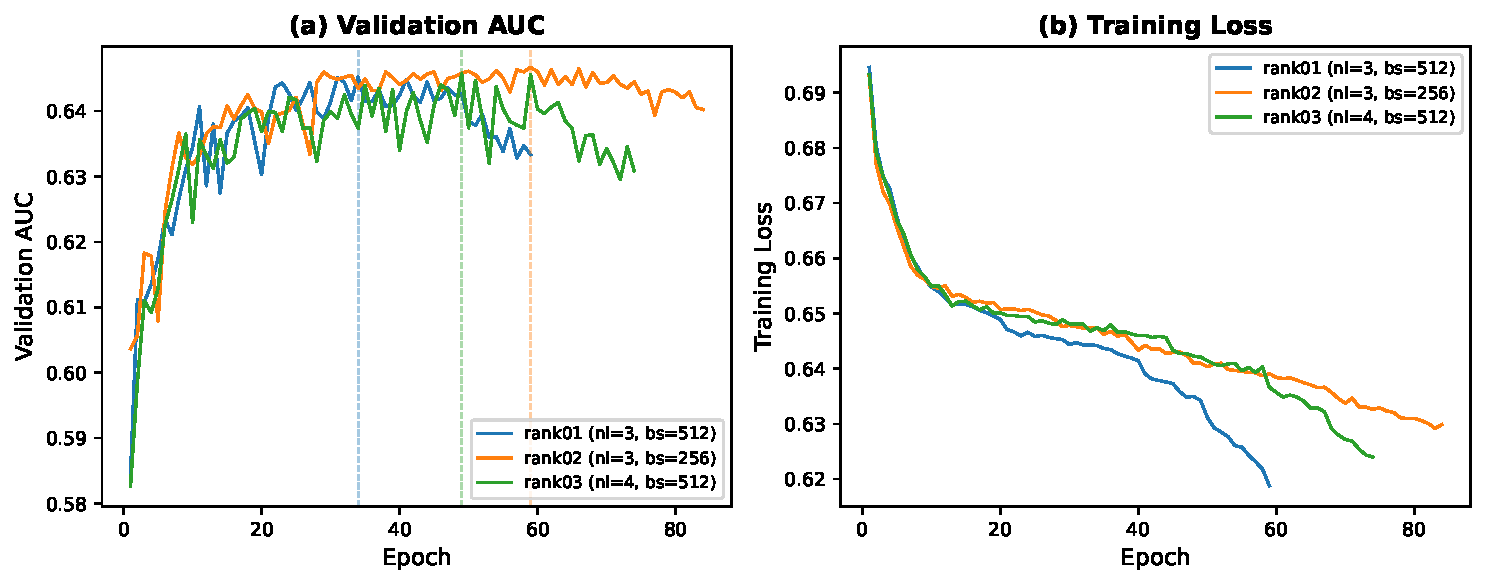
\includegraphics[width=\textwidth]{figures/training_curves.pdf}
\caption{Training dynamics for top-3 configs (200 epochs). \textbf{(a)} Val AUC vs.\ epoch. \textbf{(b)} Training loss.}
\label{fig:training_curves}
\end{figure}

\begin{figure}[H]
\centering
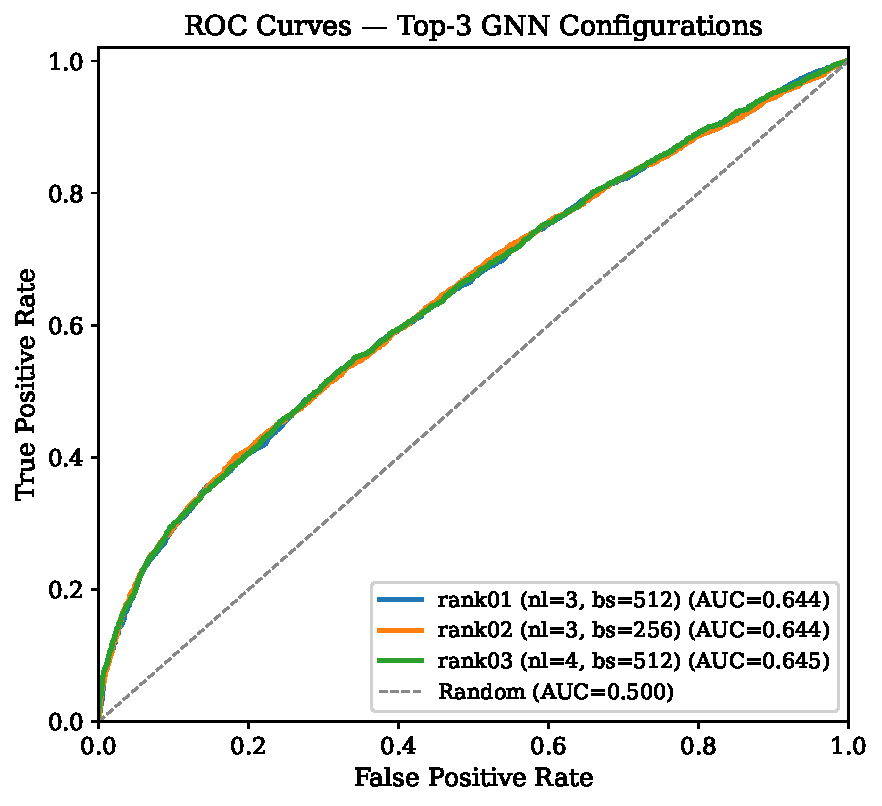
\includegraphics[width=0.55\textwidth]{figures/roc_curves_ranks.pdf}
\caption{ROC curves for the top-3 HP configurations on the held-out test set (8,715 shots). All three curves nearly overlap, consistent with their tight AUC spread (0.6437--0.6451).}
\label{fig:roc_ranks}
\end{figure}

\begin{figure}[H]
\centering
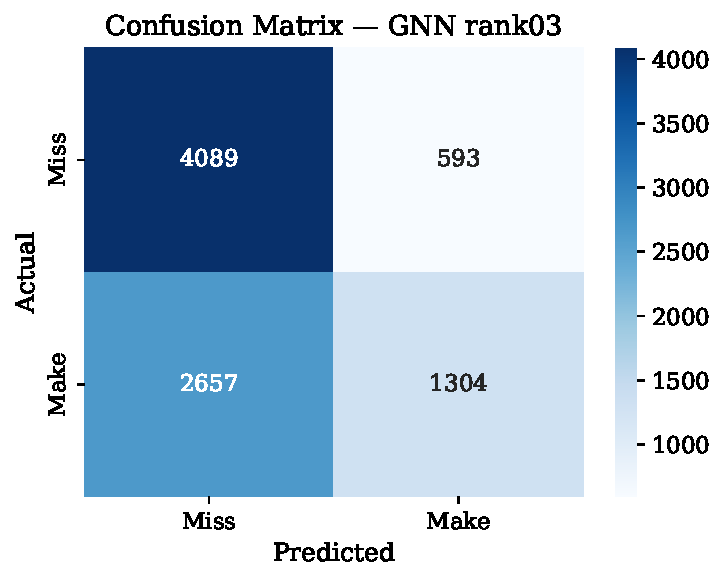
\includegraphics[width=0.45\textwidth]{figures/cm_gnn_rank03.pdf}%
\hfill%
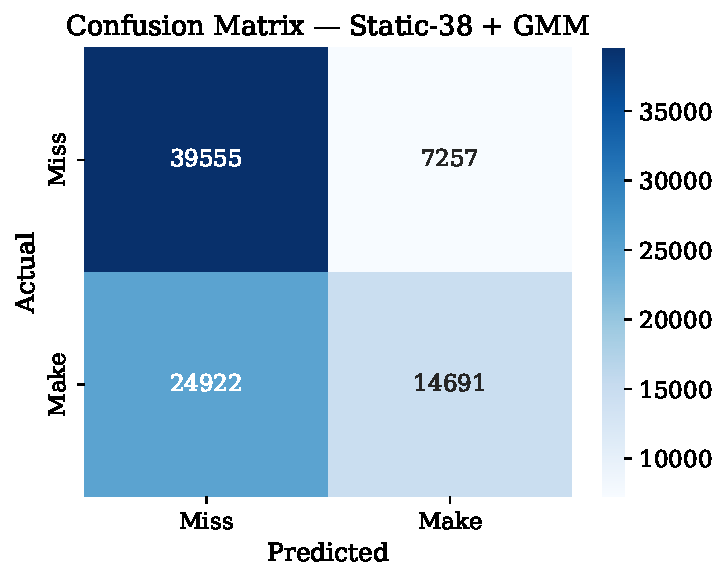
\includegraphics[width=0.45\textwidth]{figures/cm_Static_38_plus_GMM.pdf}
\caption{Confusion matrices on held-out data. \textbf{Left:} GNN rank03 (test set, 8,643 shots). \textbf{Right:} Static-38 + GMM hybrid (aggregated 5-fold CV, 86,425 shots). The hybrid achieves higher recall on makes (14,691 vs.\ 1,304 scaled) while maintaining similar precision.}
\label{fig:confusion_matrices}
\end{figure}

\begin{table}[H]
\centering
\caption{Validation--test AUC gap. Mean 0.004 confirms effective regularization.}
\label{tab:val_test_gap}
\small
\begin{tabular}{@{}lccc@{}}
\toprule
\textbf{Model} & \textbf{Val AUC} & \textbf{Test AUC} & \textbf{Gap} \\
\midrule
TemporalGRU (rank03) & 0.6457 & 0.6451 & 0.0006 \\
TemporalGRU (rank02) & 0.6467 & 0.6444 & 0.0023 \\
TemporalGRU (rank01) & 0.6452 & 0.6437 & 0.0015 \\
Variant C (dense\_long) & 0.6458 & 0.6411 & 0.0047 \\
TemporalGRU (default) & 0.6368 & 0.6346 & 0.0022 \\
Static GAT (shooter) & 0.6399 & 0.6342 & 0.0057 \\
EdgeConv & 0.6389 & 0.6311 & 0.0078 \\
SAGEConv & 0.6155 & 0.6094 & 0.0061 \\
\midrule
\textbf{Mean} & & & \textbf{0.0039} \\
\bottomrule
\end{tabular}
\end{table}

\begin{table}[H]
\centering
\caption{GMM cluster summary ($K\!=\!10$, BIC-selected). The GNN's latent space recovers NBA shot archetypes.}
\label{tab:gmm_clusters}
\small
\begin{tabular}{@{}crccccc@{}}
\toprule
\textbf{Cl.} & \textbf{$n$} & \textbf{FG\%} & \textbf{Dist (ft)} & \textbf{\% 3PT} & \textbf{Clock} & \textbf{Archetype} \\
\midrule
0 & 11,610 & 38.5 & 22.4 & 46.5 & 12.6 & Above-break 3s \\
1 & 7,755 & 41.1 & 7.1 & 0.1 & 11.5 & Paint \\
2 & 5,461 & 87.7 & 5.7 & 0.0 & 18.5 & At-rim / dunks \\
3 & 11,992 & 41.6 & 18.8 & 18.1 & 12.8 & Long 2s / some 3s \\
4 & 6,924 & 43.7 & 3.9 & 0.0 & 14.4 & Contested close \\
5 & 6,589 & 28.9 & 20.7 & 43.6 & 6.5 & Late-clock 3s \\
6 & 5,415 & 65.2 & 2.7 & 0.0 & 15.9 & Putbacks \\
7 & 6,049 & 62.0 & 5.8 & 0.7 & 13.9 & Short-range \\
8 & 12,712 & 35.0 & 21.9 & 48.4 & 11.6 & Contested 3s \\
9 & 11,918 & 46.3 & 15.2 & 7.6 & 12.4 & Mid-range \\
\bottomrule
\end{tabular}
\end{table}

\begin{figure}[H]
\centering
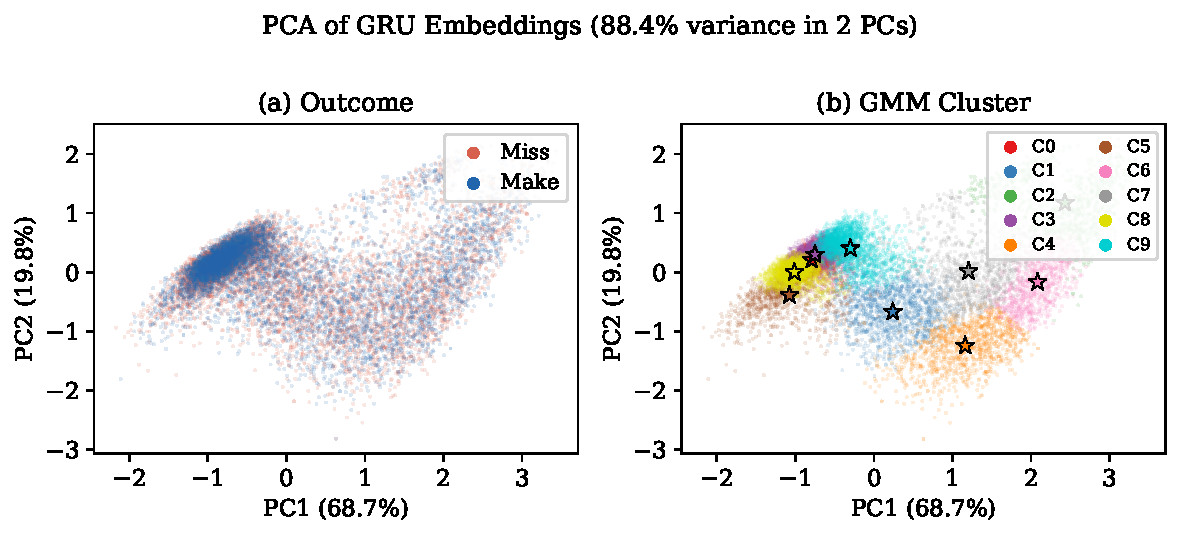
\includegraphics[width=\textwidth]{figures/pca_gmm_scatter.pdf}
\caption{PCA of GRU embeddings (88.4\% variance in 2 PCs). \textbf{(a)} By FG\%. \textbf{(b)} By GMM cluster.}
\label{fig:pca_gmm}
\end{figure}

\begin{figure}[H]
\centering
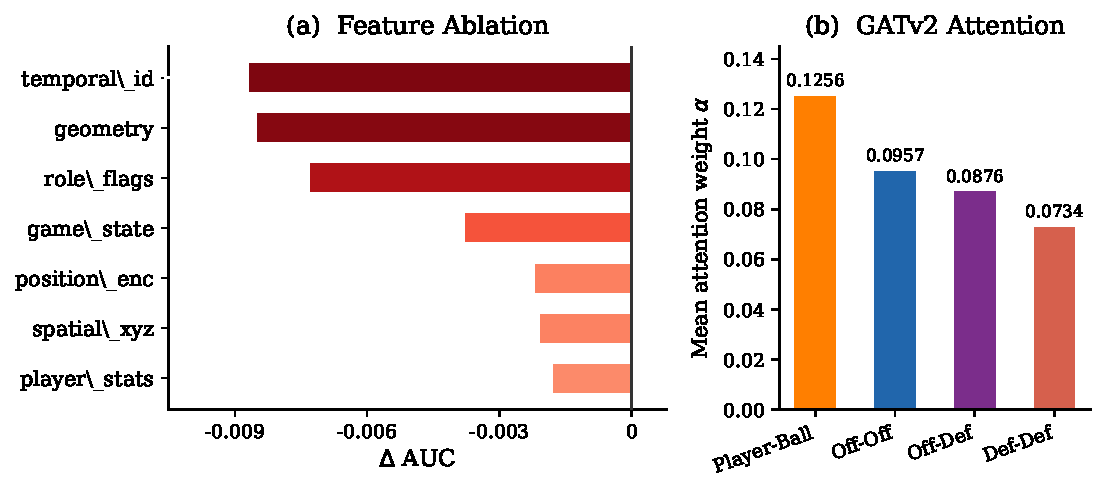
\includegraphics[width=\columnwidth]{figures/interpretability_panel.pdf}
\caption{\textbf{(a)} Feature ablation: AUC drop when each group is zeroed. Temporal ordering and geometry most critical; player stats least. \textbf{(b)} Mean GATv2 attention weight by edge type. Player-ball edges receive $\sim$1.7$\times$ more attention than D-D edges.}
\label{fig:interpretability}
\end{figure}

\begin{table}[H]
\centering
\caption{Feature ablation. $\Delta$AUC relative to full model (0.6451).}
\label{tab:ablation}
\small
\begin{tabular}{@{}lcc@{}}
\toprule
\textbf{Feature Group} & \textbf{AUC} & \textbf{$\Delta$AUC} \\
\midrule
temporal\_id (shuffle) & 0.6364 & $-$0.0087 \\
geometry (5 feat.) & 0.6366 & $-$0.0085 \\
role\_flags (3 feat.) & 0.6378 & $-$0.0073 \\
game\_state (3 feat.) & 0.6413 & $-$0.0038 \\
position\_enc (5 feat.) & 0.6429 & $-$0.0022 \\
spatial\_xyz (3 feat.) & 0.6430 & $-$0.0021 \\
player\_stats (21 feat.) & 0.6433 & $-$0.0018 \\
\bottomrule
\end{tabular}
\end{table}

\begin{table}[H]
\centering
\caption{Mean input gradient saliency ($\times 10^{-5}$) by node role and feature group (8,715 test shots).}
\label{tab:saliency}
\small
\begin{tabular}{@{}lrrrrrrr@{}}
\toprule
\textbf{Node Role} & \textbf{Role} & \textbf{Geom} & \textbf{Pos} & \textbf{TID} & \textbf{Stats} & \textbf{XYZ} & \textbf{State} \\
\midrule
Shooter  & \textbf{3.55} & 2.23 & 2.55 & 0.60 & 1.05 & 0.56 & 0.42 \\
Ball     & \textbf{3.20} & 2.12 & 1.85 & 1.28 & 0.52 & 0.81 & 0.31 \\
Defense  & \textbf{1.47} & 0.78 & 0.80 & 0.40 & 0.26 & 0.17 & 0.11 \\
Offense  & 0.82 & 0.49 & \textbf{0.47} & 0.16 & 0.19 & 0.14 & 0.11 \\
\bottomrule
\end{tabular}
\end{table}

\begin{table}[H]
\centering
\caption{Mean GATv2 attention by distance bin and edge type.}
\label{tab:attn_distance}
\small
\begin{tabular}{@{}lcccc@{}}
\toprule
\textbf{Distance} & \textbf{PB} & \textbf{OO} & \textbf{OD} & \textbf{DD} \\
\midrule
0--6 ft   & \textbf{0.128} & 0.104 & 0.098 & 0.082 \\
6--12 ft  & 0.118 & 0.092 & 0.087 & 0.071 \\
12--20 ft & 0.103 & 0.084 & 0.079 & 0.068 \\
20+ ft    & 0.110 & 0.088 & 0.085 & 0.070 \\
\bottomrule
\end{tabular}
\end{table}

\begin{table}[H]
\centering
\caption{Phase 1 results (1,745 shots). Best GNN AUC 0.594 vs.\ LR 0.614. Scaling reversed this gap.}
\label{tab:phase1}
\small
\begin{tabular}{@{}llcc@{}}
\toprule
\textbf{Model} & \textbf{Readout / Loss} & \textbf{AUC} & \textbf{F1} \\
\midrule
\multicolumn{4}{l}{\emph{Exp 1: Pooling (GAT, CE)}} \\
GAT mean$\oplus$max & concat(mean, max) & \textbf{0.594} & 0.000 \\
GAT add & sum pool & 0.505 & 0.118 \\
GAT mean & global mean & 0.476 & 0.108 \\
GAT max & global max & 0.474 & 0.233 \\
\midrule
\multicolumn{4}{l}{\emph{Exp 2: Shooter-centric}} \\
GINE mean & global mean & 0.537 & --- \\
GAT shooter & concat(shooter, mean) & 0.524 & --- \\
GINE shooter & concat(shooter, mean) & 0.485 & --- \\
\midrule
\multicolumn{4}{l}{\emph{Exp 7: Loss variants (GAT mean)}} \\
GAT + Focal $\gamma$=1.0 & CE baseline & 0.507 & --- \\
GAT + CE & CE & 0.476 & --- \\
GAT + LS $\alpha$=0.10 & label smooth & 0.476 & --- \\
GAT + LS $\alpha$=0.05 & label smooth & 0.447 & --- \\
\bottomrule
\end{tabular}
\end{table}

% =============================================================================
\clearpage

\section{Appendix: Additional Details}
\label{app:additional_details}

\paragraph{GINEConv.}
\hypertarget{app:gineconv}{}
\citep{hu2020gine} extends the GIN framework \citep{xu2019gin} with edge features:
$\mathbf{h}_i' = \text{MLP}\!\big((1+\epsilon)\,\mathbf{h}_i + \sum_{j \in \mathcal{N}(i)} \text{ReLU}(\mathbf{h}_j + \mathbf{e}_{ij})\big)$,
where $\epsilon$ is a learnable parameter. GINE sums all neighbor contributions with equal weight, so it cannot distinguish high-relevance neighbors (e.g., the closest defender) from low-relevance ones. This uniform aggregation limits expressiveness compared to attention-based models (AUC 0.6242; Table~\ref{tab:arch_comparison}).

\paragraph{SAGEConv.}
\hypertarget{app:sageconv}{}
\citep{hamilton2017sage} applies mean aggregation without edge features:
$\mathbf{h}_i' = \mathbf{W}_1\mathbf{h}_i + \mathbf{W}_2 \cdot \text{MEAN}_{j \in \mathcal{N}(i)}[\mathbf{h}_j]$.
By ignoring edge attributes, SAGEConv cannot leverage spatial relationships between players---problematic when defender distance is a primary signal. This limitation is reflected in its poor performance (AUC 0.6094, F1 0.143; Table~\ref{tab:arch_comparison}).

\paragraph{EdgeConv.}
\hypertarget{app:edgeconv}{}
\citep{wang2019edgeconv}, designed for point clouds, captures relative geometry via:
$\mathbf{h}_i' = \max_{j \in \mathcal{N}(i)} \text{MLP}([\mathbf{h}_i \| \mathbf{h}_j - \mathbf{h}_i])$,
where $\mathbf{h}_j - \mathbf{h}_i$ encodes relative positioning between neighbors. Max aggregation retains only the most extreme neighbor signal, which limits expressiveness compared to attention-based weighting but validates that relative spatial relationships carry predictive signal (AUC 0.6311; Table~\ref{tab:arch_comparison}).

\paragraph{Readouts.}
\hypertarget{app:readouts}{}
After $L$ layers of message passing, we collapse all 11 node embeddings $\{\mathbf{h}_i'\}$ into a single fixed-size vector representing the entire court configuration (edge information is already absorbed into node embeddings during message passing). We test five strategies: global mean, max, and sum pooling; mean$\oplus$max concatenation (which captures both the ``average'' and ``extreme'' court configuration); and a shooter-centric readout that concatenates the shooter node's embedding with the scene mean, explicitly isolating the shooter's learned representation.

\paragraph{Loss Functions.}
\hypertarget{app:losses}{}
\textbf{Cross-entropy} (CE): $\mathcal{L} = -\sum_i [y_i \log \hat{p}_i + (1\!-\!y_i)\log(1\!-\!\hat{p}_i)]$, the standard objective for binary classification.
\textbf{Label smoothing} replaces hard targets with $(1\!-\!\alpha)\cdot\mathbf{y}_{\text{one-hot}} + \alpha/C$, preventing overconfident predictions. We test $\alpha \in \{0.05, 0.10\}$.
\textbf{Focal loss} \citep{lin2017focal} down-weights well-classified examples: $\mathcal{L}_{\text{FL}} = -(1-\hat{p}_t)^\gamma \log \hat{p}_t$, where $\hat{p}_t$ is the predicted probability for the true class and $\gamma > 0$ controls the focusing strength. We test $\gamma \in \{0.5, 1.0, 2.0\}$.

\paragraph{Node \& Edge Features.}
\hypertarget{app:features}{}
Each node carries 41 features: $(x,y,z)$ coordinates; role flags (has\_ball, is\_offense, is\_player\_node); geometry (dist\_to\_rim, dist\_to\_ball\_handler, angle\_to\_basket, dist\_to\_3pt, num\_nearby\_def); game state (quarter, game\_clock, shot\_clock, timestamp); 5-dim sinusoidal position encoding; and 21 player career statistics (FG\%, distance-bucket percentages, assist rates, etc.). Only 3 statistics are manually normalized: age$/40$, avg\_dist$/30$, games$/82$; all other node features---coordinates, distances, angles, clocks, counts, percentages---are used raw with no global normalization. Each edge carries 9 features: relative displacement $(x_{\text{rel}}, y_{\text{rel}})$, Euclidean distance, edge angle, and a 5-dim one-hot encoding the edge type (offense--offense, offense--defense, defense--defense, player--ball, temporal).

% =============================================================================
\clearpage
\bibliographystyle{acl_natbib}
\bibliography{references}

\end{document}
